
Recent methodological developments have improved the statistical robustness and the degree of automation of relative binding free-energy (RBFE) calculations, which are now routinely applied in drug discovery projects in industry. 
\cite{Cournia2017,Cournia2020, Meier2021, Armacost2020c, Barros2022,
       Heinzelmann2021, Gapsys2020, Jespers2019, Raman2020,
       Christ2014, Gao2018, Tielker2021, Loeffler2018}
       %reviews - FE methods/ usage in industry
       %Methods - automation, accuracy
       %FE benchmark - challenges
%
A free-energy calculation provides information about the relative populations of multiple end-states in equilibrium. Examples are drug design, where the end-states represent the different ligands that bind to a protein, \cite{Christ2009, Riniker2011, Wang2015, Wang2017, Aldeghi2016, Sidler2016,Yu2017, Jespers2019,Jiang2019, Paulsen2020} or protein engineering, where the end-states correspond to the different amino acids considered for one position in the protein.\cite{Shobana2000, Bieler2015B, Jespers2019B}
Each free-energy calculation involves the choice of a sampling approach, a free-energy estimator (e.g. thermodynamic integration (TI),\cite{Kirkwood1935} the Zwanzig equation,\cite{Zwanzig1954} or Bennett's acceptance ratio (BAR)\cite{Bennett1976}), and a representation of the end-states (i.e., molecules or substructures of molecules) during the simulation.

%%% The solutions in application
Several possible representations have been proposed in the past to build a coordinate and topology space of the end-states. 
Historically, two approaches emerged, which were termed ``single topology'' \cite{Pearlman1991, Pearlman1994} and ``dual topology'' \cite{Pearlman1991, Gao1989}.
Unfortunately, the terminology is not always clear in the literature and these terms are used ambiguously.\cite{Boresch1999, Rocklin2013, Fleck2021}
To distinguish the different representation options, we propose here a terminology based on the difference in the respective coordinate space (Figure \ref{fig:Topology Types}). These definitions may differ from the historical ones. The single topology approach contains a single set of coordinates for both end states. In contrast,  the dual topology approach involves a separate set of coordinates for each end state. The two approaches can be seen as opposite extremes. Three sub-variants of the dual topology approach can be found in the literature: linked, separated and unconstrained.
In addition, a ``hybrid topology'' approach was recently described,\cite{Jiang2019} which presents an intermediate between the single and dual approaches (Figure \ref{fig:Topology Types}). This scheme has been used in many studies for binding free energy calculations before but not called hybrid topology. In protein engineering however Shobana \textit{et al.} used a similar approach called hybrid topology.\cite{Shobana2000} The different representations vary with respect to sampling efficiency and the capability of handling complex transformations.

\begin{figure}[h!]
    \centering
    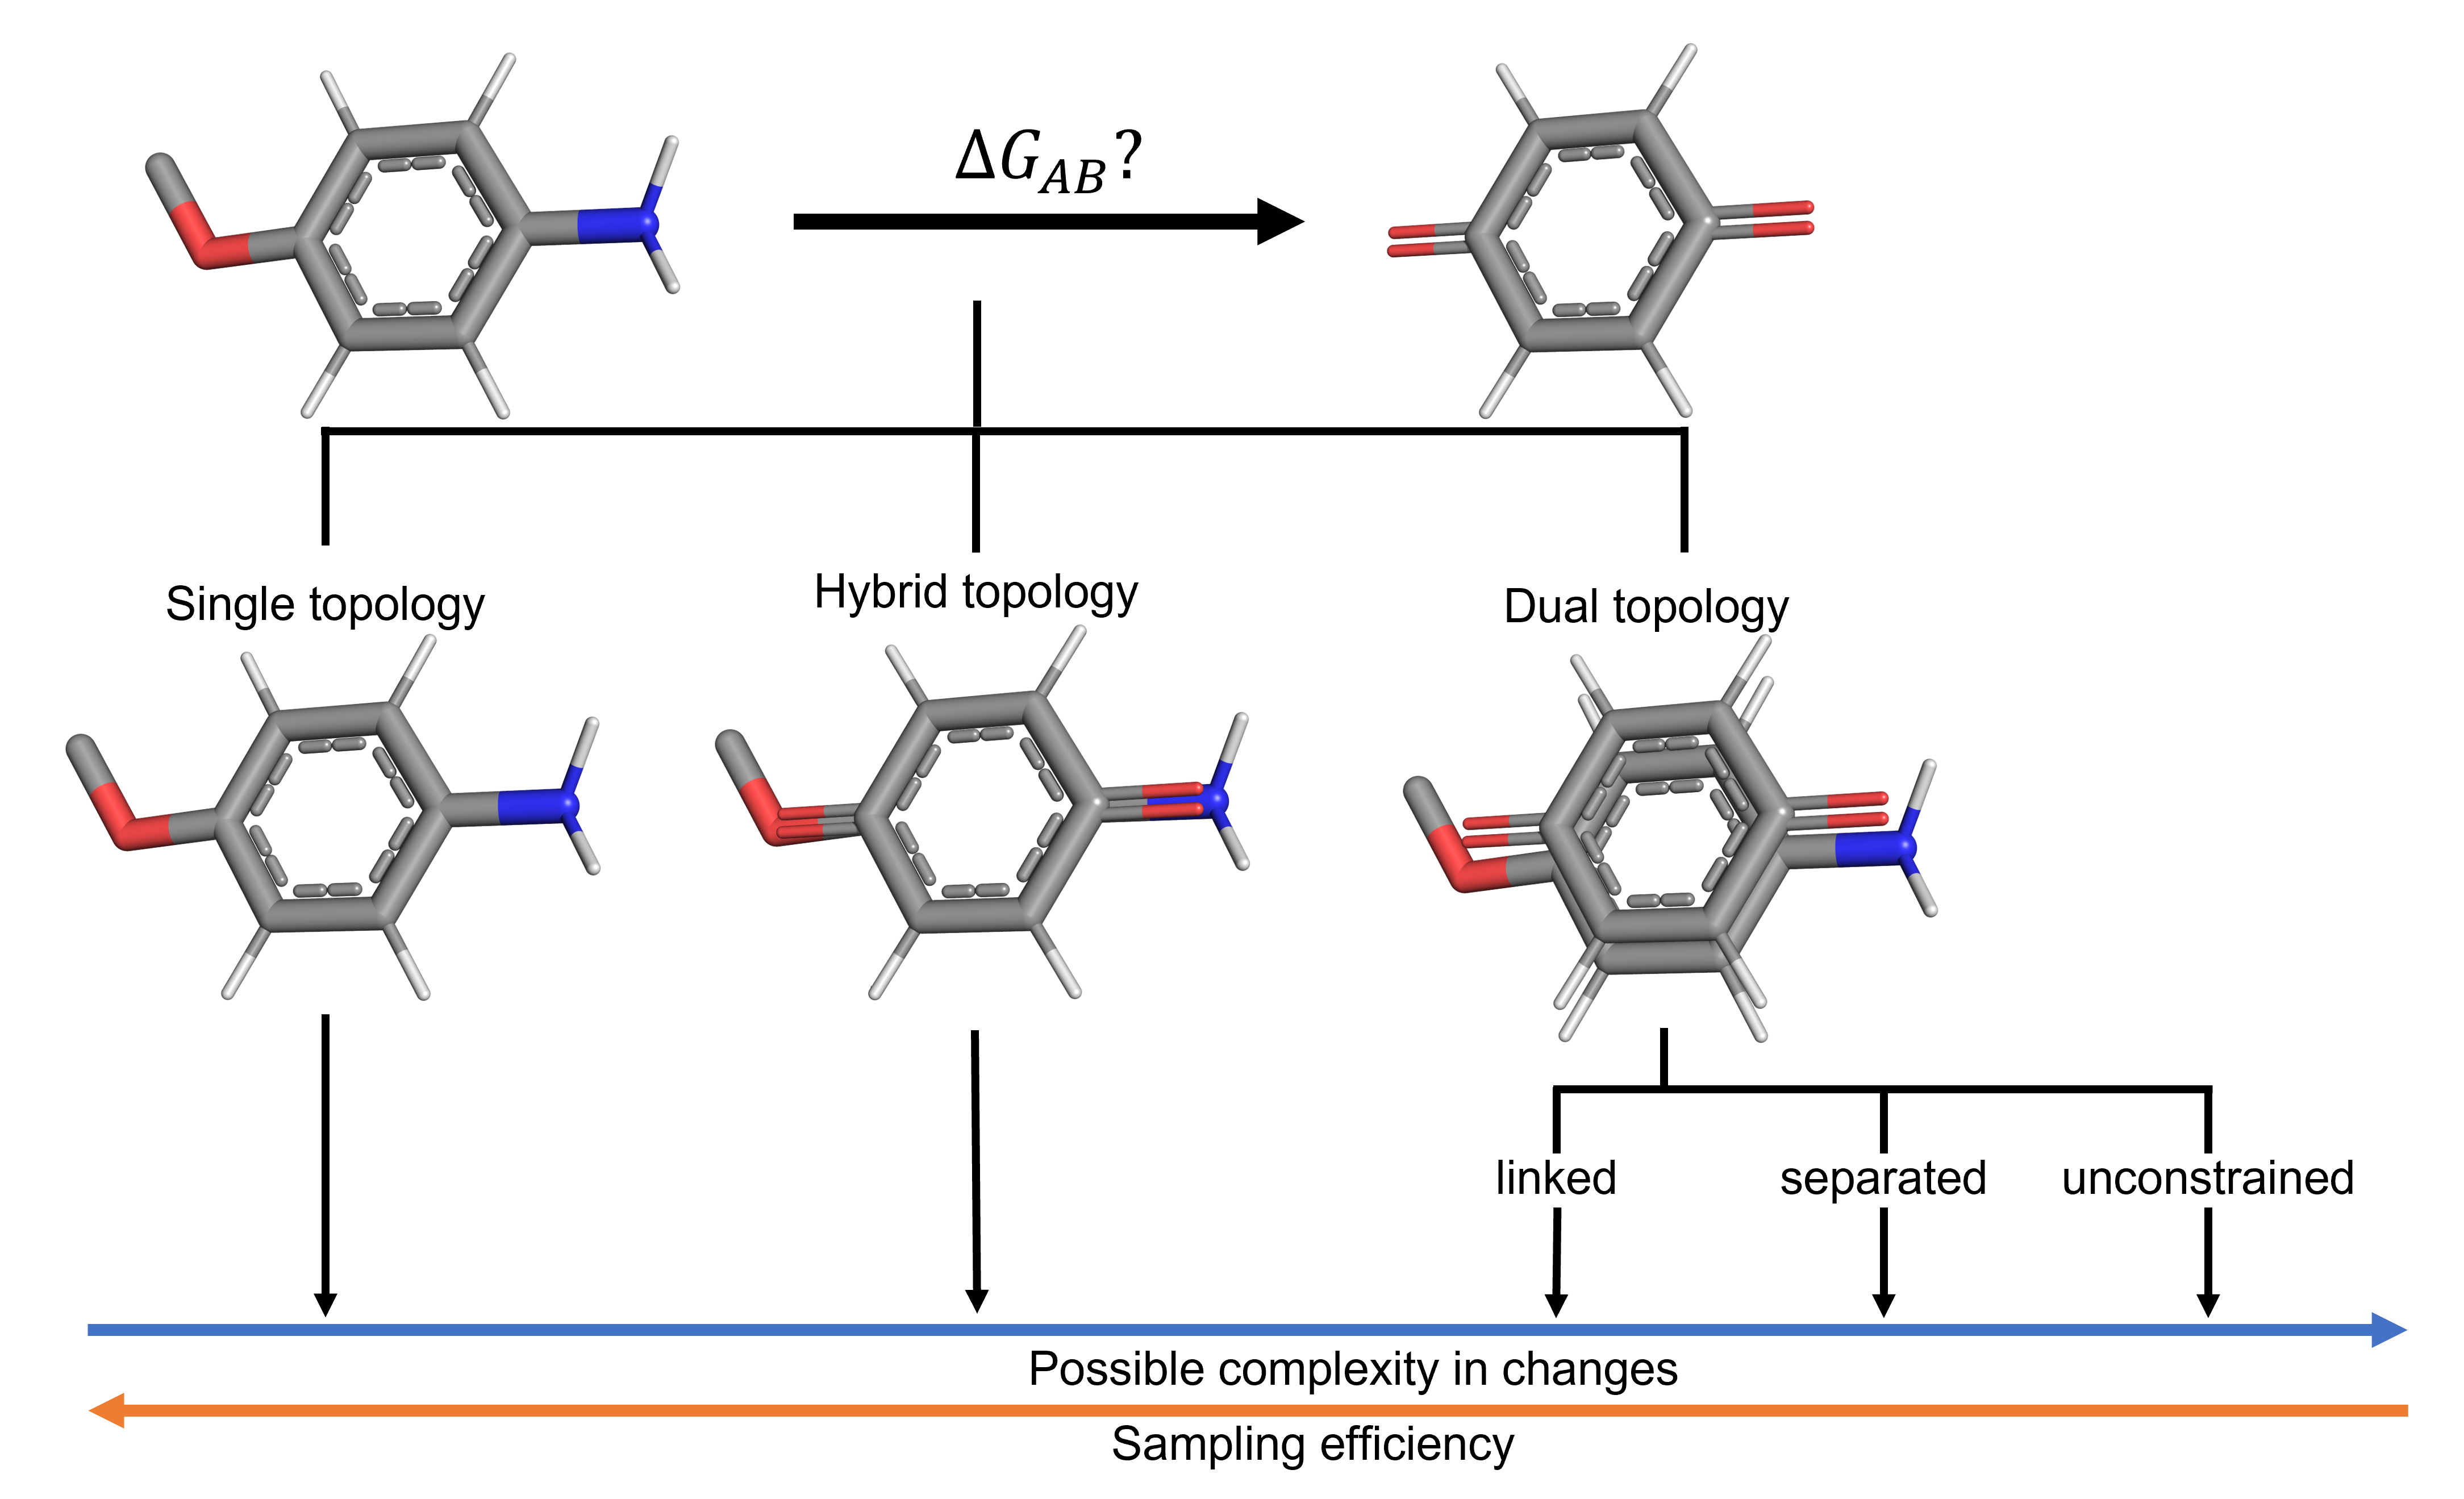
\includegraphics[width=\linewidth]{fig/theory/landscape_of_simulationApproaches.png}
    \caption{Three end-state representations can be distinguished based on the coordinate space. The ``single topology'' approach (left) contains a single set of coordinates for all end-states. The ``dual topology'' approach contains separate sets of coordinates for each end state (right). The ``hybrid topology'' approach (middle) combines atoms of common substructures into one coordinate set, while atoms that differ between the end-states are represented separately. It is therefore an intermediate between the two other representations. The dual topology approach can be further subdivided into three sub-variants: linked, separated, and unconstrained. The linked dual topology approach is closest to the single topology approach, as the coordinate overlap between the end-states is ensured with direct spatial restraints (e.g. distance restraints). The separated variant is connecting the molecules indirectly by restraining them spatially to the same area, whereas the unconstrained variant does not restrain the molecules at all and is therefore also the most difficult to sample.}
    \label{fig:Topology Types}
\end{figure}

%%%% automation
With the high-throughput application of RBFE calculations comes the need for automation.\cite{Christ2014} While there exist tools such as FESetup,\cite{Loeffler2015} ProtoCaller,\cite{Suruzhon2020} SMArt,\cite{Petrov2021} or LOMAP,\cite{Liu2013} to automatically set up single-topology RBFE calculations, the dual topology approaches are in principle the easiest to automate as any alchemical molecule transformation can be realized without requiring atom mapping.\cite{Rocklin2013}
For the unconstrained dual topology variant, an automatic set-up procedure is available in the packages pyAutoFEP\cite{Carvalho2021} and FEW\cite{Homeyer2013}.
When representing the end-states with a linked dual topology approach, the set-up is more difficult than in the unconstrained case as the distance restraints between the molecules need to be chosen.
For example, the QligFEP pipeline\cite{Jespers2019} provides an automatic system generation for the linked dual topology approach, where the distance restraints are placed in the perturbed common substructure of the end-states. These distance restraints only become active if the restrained atoms surpass a distance of $0.02~$ nm.
However, for more complex transformations (e.g. in scaffold hopping), a more flexible approach is needed to select the optimal distance restraints between molecules.

%outlook
In this work, we present a greedy algorithm to select optimal distance restraints for RBFE calculations with the linked dual topology approach, which is also applicable to molecule pairs without a common core. In addition, the algorithm is extended to solve the same problem for multi-state RBFE methods such as enveloping distribution sampling (EDS)\cite{Christ2007,Christ2008} and multi-site $\lambda$-dynamics,\cite{Knight2011} resulting in a linked multi-topology approach. Finally, we analyze the sampling behavior and performance of the approach for the calculation of relative hydration free energies. The algorithm is implemented in a Python package\\ (\textit{https://github.com/rinikerlab/restraintmaker}), which can be used as a scripting library or with a GUI inside PyMOL. \cite{Delano2020}